% ════════════════════════════════════════════
% 5. 模型预测与效应测算（对应赛题 2.4）
% ════════════════════════════════════════════
\section{模型预测与效应测算（对应 2.4）}

\subsection{三个新观测的预测（对应 2.4）}

题面要求给出新观测的预测结果。取三种有代表性的投放组合：付费的图片帖（主题 1）、自然帖里的视频帖（主题 1）、自然帖的主题 2，其余条件取代表性画像（7 月、周四、上午、粉丝 129,600），用最终模型 M2 的系数在对数尺度预测，再经 Duan 烟雾因子还原到曝光次数，区间由 1000 次参数模拟给出（表\ref{tab:newpred}）。三类组合的预测曝光分别为 56,364 次、197,157 次与 24,927 次，区间宽度差异明显：视频帖的区间上限是下限的 5.5 倍，原因是其参照样本只有 7 条；因此新观测若落在视频类型上，只能给出量级判断，不适合作为预算依据。

{\small
\begin{longtable}{>{\centering\arraybackslash}p{0.280\textwidth}>{\centering\arraybackslash}p{0.160\textwidth}>{\centering\arraybackslash}p{0.200\textwidth}>{\centering\arraybackslash}p{0.180\textwidth}>{\centering\arraybackslash}p{0.180\textwidth}}
  \caption{三个代表性新观测的预测曝光与区间}
  \label{tab:newpred} \\
  \toprule
  新观测 & 参照样本量 & 预测曝光（次） & 95\%CI 下限 & 95\%CI 上限 \\
  \midrule
  \endfirsthead
  \caption{三个代表性新观测的预测曝光与区间（续）} \\
  \toprule
  新观测 & 参照样本量 & 预测曝光（次） & 95\%CI 下限 & 95\%CI 上限 \\
  \midrule
  \endhead
  \bottomrule
  \endfoot
  付费（付费） & 139 & 56,364 & 36,172 & 87,327 \\
  Video（内容类型） & 7 & 197,157 & 83,333 & 456,747 \\
  主题2（内容主题） & 130 & 24,927 & 15,171 & 38,718 \\
\end{longtable}
}


\subsection{付费带来的额外曝光（对应 2.4.1）}

题面要求在内容类型、发帖时段与粉丝量相同的条件下比较付费与非付费。本文的最终模型以月份固定效应吸收粉丝规模的时间趋势（第 3.3 节），因此“粉丝量相同”由“同月”代理，其余条件由模型中的类型与时段哑变量固定；文案与文案之间只差付费标记。系数的经济含义通过三个层次还原到曝光尺度。第一层用 $\exp(\beta)-1$ 给出百分比效应；第二层用 Duan 烟雾因子把对数尺度预测还原为曝光次数，在代表性画像（Photo、主题 1、7 月、周四、上午、粉丝 129,600）上计算反事实；第三层对 500 条帖子逐条反事实并取平均，得到样本平均处理效应。表\ref{tab:paid}给出付费效应的三层结果：系数 0.337 对应 40.1\% 的提升，代表性画像上自然帖子预期曝光 40,221 次、付费帖子 56,364 次，差值 16,142 次；全样本平均处理效应为 10,907 次。原始数据的中位数比（1.438）与模型结果（1.401）接近，说明调整前后结论稳定。

{\small
\begin{longtable}{>{\centering\arraybackslash}p{0.420\textwidth}>{\centering\arraybackslash}p{0.200\textwidth}>{\centering\arraybackslash}p{0.190\textwidth}>{\centering\arraybackslash}p{0.190\textwidth}}
  \caption{付费投放的曝光效应测算}
  \label{tab:paid} \\
  \toprule
  指标 & 估计值 & 95\%CI下限 & 95\%CI上限 \\
  \midrule
  \endfirsthead
  \caption{付费投放的曝光效应测算（续）} \\
  \toprule
  指标 & 估计值 & 95\%CI下限 & 95\%CI上限 \\
  \midrule
  \endhead
  \bottomrule
  \endfoot
  M2 付费系数 β & 0.3374 & 0.1025 & 0.5723 \\
  exp(β)−1（\%） & 40.1325 & 10.7962 & 77.2364 \\
  代表性画像：
自然帖子预测曝光 & 40,221 & 25,282 & 62,189 \\
  代表性画像：
付费帖子预测曝光 & 56,364 & 36,172 & 87,327 \\
  代表性画像：
差值（次） & 16,142 & 4,543 & 33,467 \\
  代表性画像：
倍数 & 1.4013 & 1.1036 & 1.753 \\
  全样本 ATE：
差值（次） & 10,907 & 3,138 & 20,195 \\
  全样本 ATE：
倍数 & 1.4013 & 1.1036 & 1.7531 \\
  原始数据：
付费组中位曝光 & 12,060 & — & — \\
  原始数据：
自然组中位曝光 & 8,387 & — & — \\
  原始数据：
中位数比 & 1.4379 & — & — \\
  原始数据：
均值比 & 1.4051 & — & — \\
\end{longtable}
}


\subsection{视频相对图片的曝光倍数（对应 2.4.2）}

在投放状态、月份与粉丝量相同的条件下，载体形式由 Photo 换成 Video 的系数为 1.590，按 $\exp(\beta)$ 还原为 4.90 倍（95\% 区间 2.23--10.79），即同样的投放条件下视频帖的曝光约为图片帖的五倍。表\ref{tab:type}同时给出 Status 与 Link：Status 是 Photo 的 3.17 倍（2.49--4.04），Link 与 Photo 无显著差异（倍数 1.13，区间跨 1）。需要标注的是视频帖仅 7 条，其区间宽度是 Photo 组的 10 倍以上，倍数只能作为方向性证据，不能直接当作预算系数。

{\small
\begin{longtable}{>{\centering\arraybackslash}p{0.180\textwidth}>{\centering\arraybackslash}p{0.140\textwidth}>{\centering\arraybackslash}p{0.120\textwidth}>{\centering\arraybackslash}p{0.140\textwidth}>{\centering\arraybackslash}p{0.180\textwidth}>{\centering\arraybackslash}p{0.180\textwidth}}
  \caption{内容类型相对 Photo 的曝光差异}
  \label{tab:type} \\
  \toprule
  对比 & 系数 & p值 & 倍数 & 倍数CI下限 & 倍数CI上限 \\
  \midrule
  \endfirsthead
  \caption{内容类型相对 Photo 的曝光差异（续）} \\
  \toprule
  对比 & 系数 & p值 & 倍数 & 倍数CI下限 & 倍数CI上限 \\
  \midrule
  \endhead
  \bottomrule
  \endfoot
  Video vs Photo & 1.5896 & 0.0001 & 4.9017 & 2.2262 & 10.7925 \\
  Status vs Photo & 1.1538 & 0 & 3.1702 & 2.4869 & 4.0412 \\
  Link vs Photo & 0.1215 & 0.6428 & 1.1292 & 0.6750 & 1.8891 \\
\end{longtable}
}


\subsection{内容主题对曝光的影响（对应 2.4.3）}

内容主题的联合 Wald 检验 $p=0.0018$，说明三个主题的曝光水平并不同质。两两对比中，主题 2 比主题 1 低 38.0\%（$p=0.0004$），主题 3 比主题 1 低 27.0\%（$p=0.019$），主题 2 与主题 3 之间无显著差异（$p=0.65$）。也就是说，主题 1 的文案在同等条件下获得的曝光最高，主题 2 与主题 3 依次次之，但后两者彼此难以区分。

\begin{figure}[htbp]
  \centering
  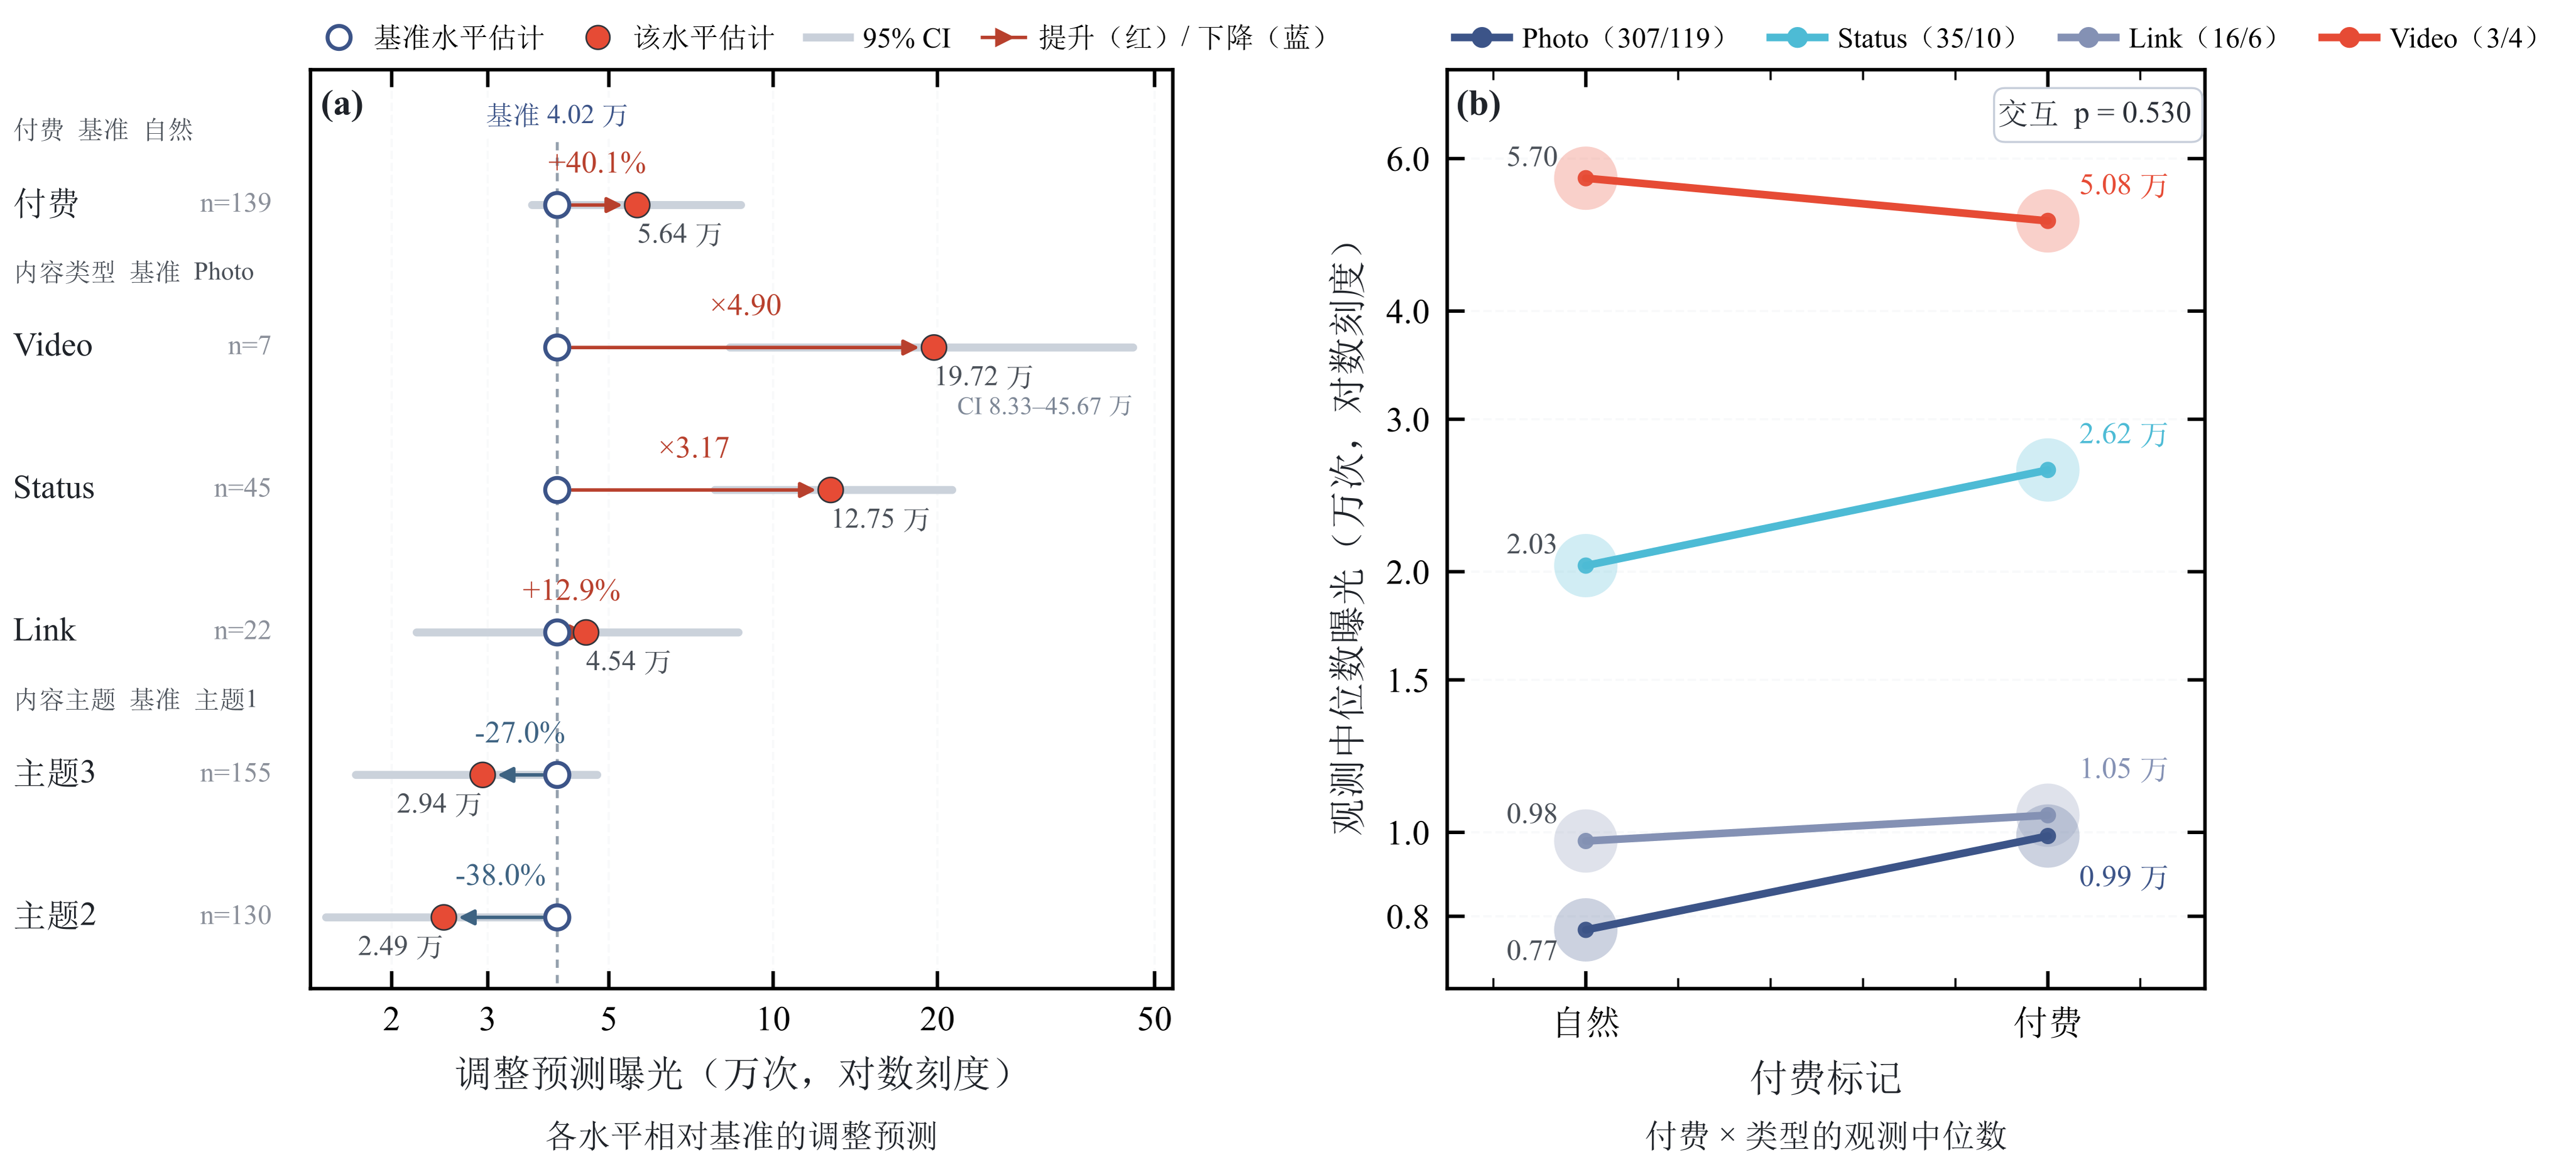
\includegraphics[width=0.76\textwidth]{../求解/问题四/结果/图11_调整预测效应.png}
  \caption{调整后的预测曝光：付费、内容类型与内容主题}
  \label{fig:adj}
\end{figure}

图\ref{fig:adj}把三组调整预测画在同一画布：付费组相对自然组提升 40.1\%，视频组 19.72 万次但区间最宽，主题 2 最低（2.49 万次）；右下图显示付费与类型的交互检验 $p=0.530$，交互项不显著，效应以主效应为主。

\subsection{稳健性检验与异质性}

六种模型设定下的效应见表\ref{tab:robust}与图\ref{fig:robust}。付费提升幅度在 37.4\%--49.6\% 之间，视频倍数在 3.52--5.41 之间，全部设定下方向一致、显著性不变；M3 与 M4 因剔除月份而略有上移，Huber 稳健回归与 Gamma GLM 给出更保守的估计，说明结论不依赖单一估计方法。

{\small
\begin{longtable}{>{\centering\arraybackslash}p{0.200\textwidth}>{\centering\arraybackslash}p{0.120\textwidth}>{\centering\arraybackslash}p{0.090\textwidth}>{\centering\arraybackslash}p{0.090\textwidth}>{\centering\arraybackslash}p{0.140\textwidth}>{\centering\arraybackslash}p{0.090\textwidth}>{\centering\arraybackslash}p{0.090\textwidth}>{\centering\arraybackslash}p{0.120\textwidth}}
  \caption{六种模型设定下的效应稳健性}
  \label{tab:robust} \\
  \toprule
  设定 & 付费提升（\%） & 提升下限 & 提升上限 & Video 倍数 & 倍数下限 & 倍数上限 & $X_3$ 联合 $p$ \\
  \midrule
  \endfirsthead
  \caption{六种模型设定下的效应稳健性（续）} \\
  \toprule
  设定 & 付费提升（\%） & 提升下限 & 提升上限 & Video 倍数 & 倍数下限 & 倍数上限 & $X_3$ 联合 $p$ \\
  \midrule
  \endhead
  \bottomrule
  \endfoot
  M1 全模型 & 40.0891 & 10.7199 & 77.2487 & 4.8944 & 2.2284 & 10.7499 & 0.0019 \\
  M2 月份固定效应 & 40.1325 & 10.8626 & 77.1301 & 4.9017 & 2.2307 & 10.7708 & 0.0018 \\
  M3 仅logX1 & 49.6482 & 18.5385 & 88.9225 & 5.2503 & 2.5022 & 11.0164 & 0.0052 \\
  M4 logX1+线性月份 & 47.137 & 15.8511 & 86.8717 & 5.4076 & 2.6179 & 11.17 & 0.0030 \\
  Huber 稳健回归 & 37.4423 & 13.2266 & 66.837 & 5.3838 & 2.5841 & 11.2168 & 0.0045 \\
  Gamma GLM（log 链接） & 44.8408 & 9.4426 & 91.6882 & 3.518 & 1.7216 & 7.1886 & 0.0001 \\
\end{longtable}
}


\begin{figure}[p]
  \centering
  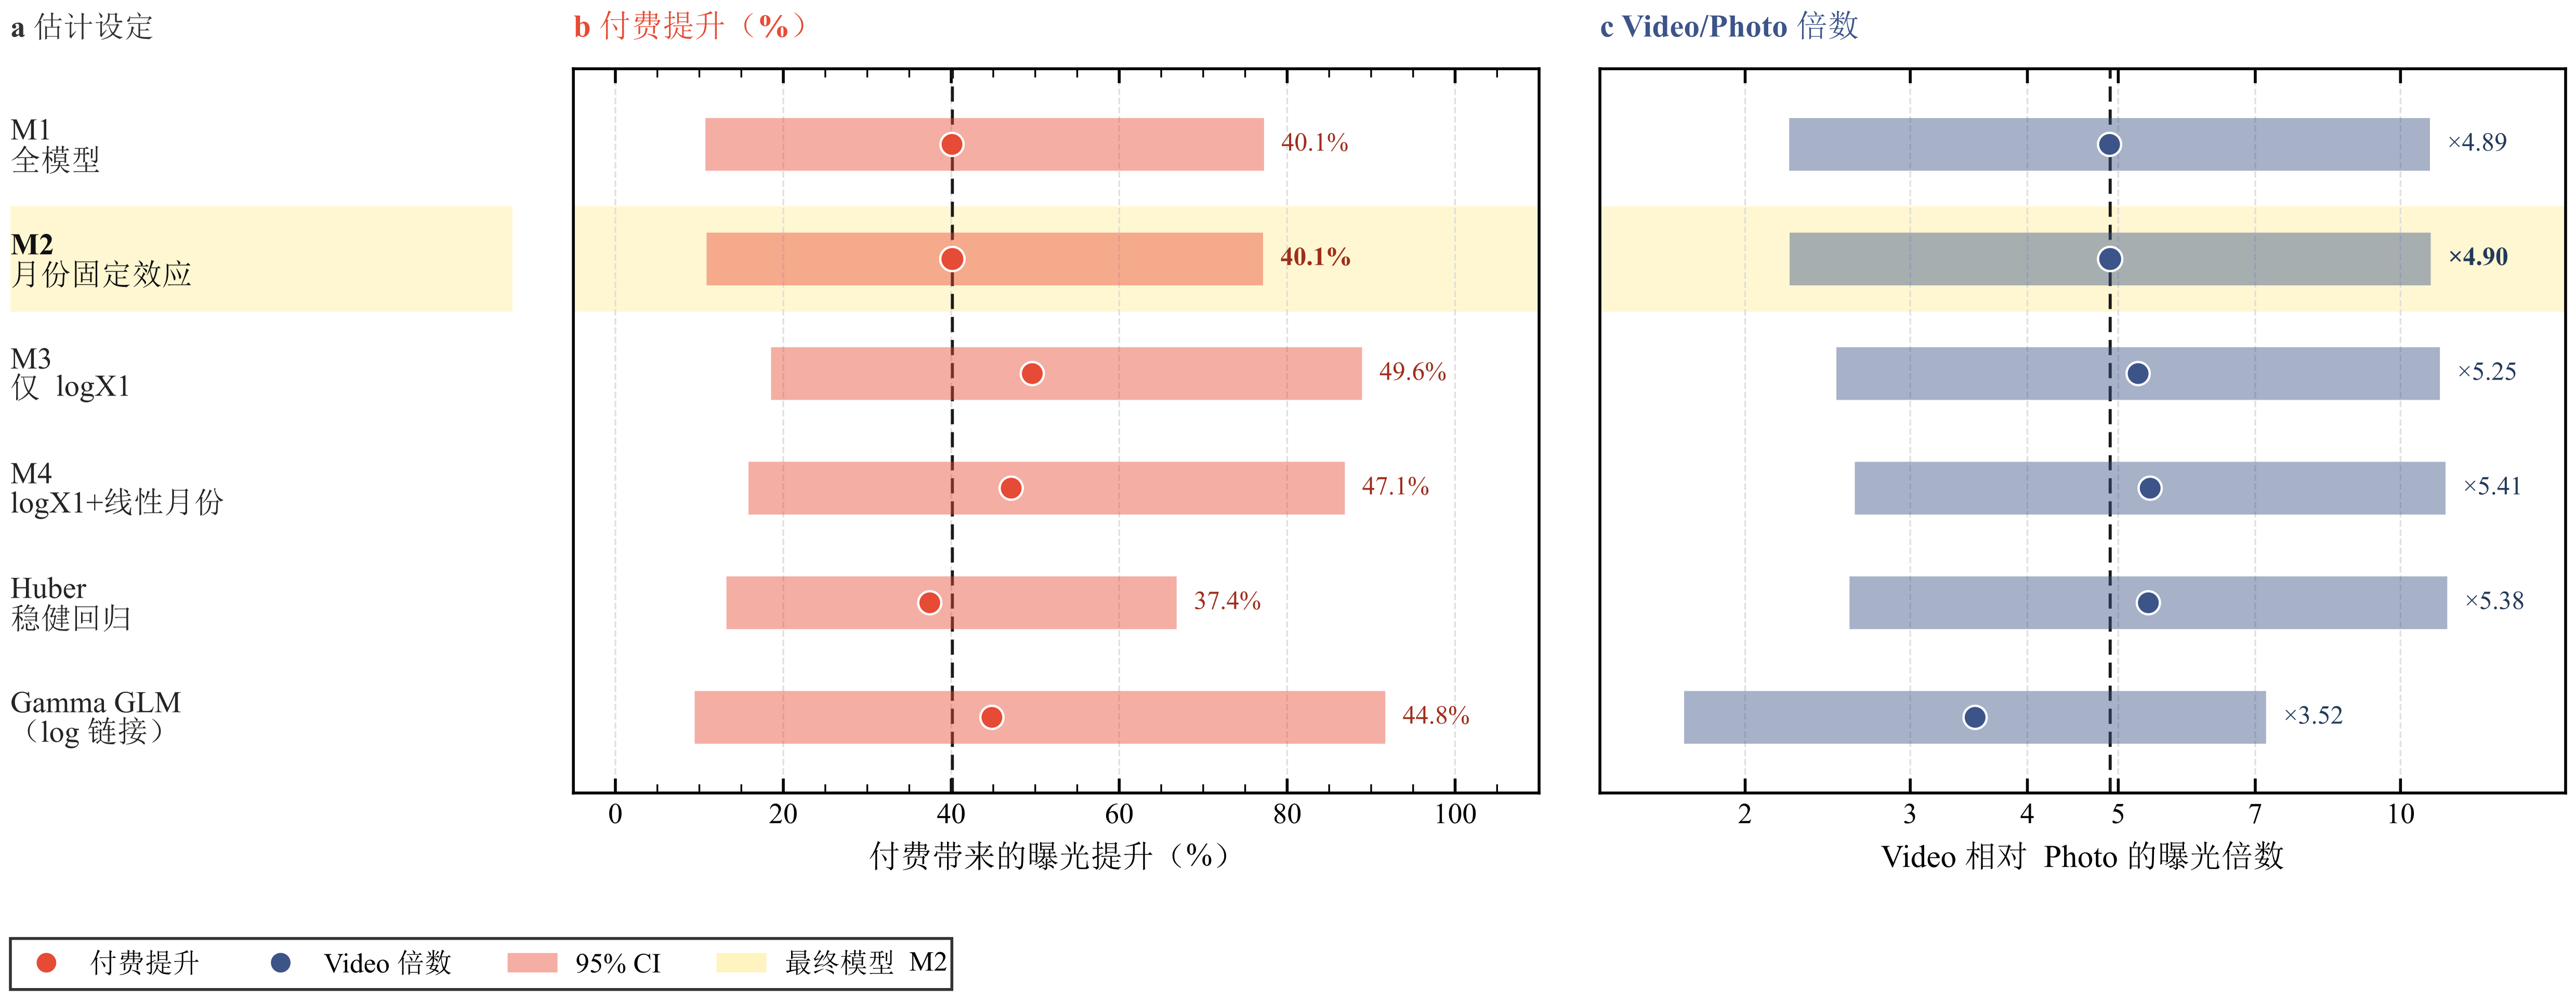
\includegraphics[width=0.60\textwidth]{../求解/问题四/结果/图12_效应稳健性.png}
  \caption{六种设定下的付费提升幅度与视频曝光倍数}
  \label{fig:robust}
\end{figure}

按子样本重估同一规格模型，结果见表\ref{tab:hetero}。类型与时段内部的付费效应没有显著差异（组内 $p=0.531$、$p=0.474$），但内容主题内部存在异质性（组内 $p=0.036$）：主题 1 的付费系数为 0.571（$p=0.008$），主题 3 仅为 0.018（$p=0.911$）。这意味着“付费提升四成”这一平均效应主要由主题 1 的帖子贡献，主题 3 的帖子几乎无法通过付费获得额外曝光。视频（7 条）与链接（22 条）子样本的自由度过低，其系数只能标注为参考，不能用于决策。

{\small
\begin{longtable}{>{\centering\arraybackslash}p{0.150\textwidth}>{\centering\arraybackslash}p{0.160\textwidth}>{\centering\arraybackslash}p{0.090\textwidth}>{\centering\arraybackslash}p{0.140\textwidth}>{\centering\arraybackslash}p{0.130\textwidth}>{\centering\arraybackslash}p{0.130\textwidth}>{\centering\arraybackslash}p{0.120\textwidth}}
  \caption{付费效应的子样本异质性}
  \label{tab:hetero} \\
  \toprule
  分组 & 子样本 & $N$ & 系数 & 下限 & 上限 & $p$ \\
  \midrule
  \endfirsthead
  \caption{付费效应的子样本异质性（续）} \\
  \toprule
  分组 & 子样本 & $N$ & 系数 & 下限 & 上限 & $p$ \\
  \midrule
  \endhead
  \bottomrule
  \endfoot
  全样本 & 全样本 & 500 & 0.3374 & 0.1025 & 0.5723 & 0.0050 \\
  帖子类型 & Photo & 426 & 0.3891 & 0.1289 & 0.6492 & 0.0035 \\
  帖子类型 & Status & 45 & 0.3526 & -0.2869 & 0.9921 & 0.2669 \\
  帖子类型 & Link & 22 & -0.5491 & -2.9451 & 1.8469 & 0.6207 \\
  帖子类型 & Video & 7 & -0.1900 & -2.6262 & 2.2463 & 0.8490 \\
  内容主题 & 主题 1 & 215 & 0.5700 & 0.1528 & 0.9872 & 0.0077 \\
  内容主题 & 主题 2 & 130 & 0.4251 & -0.0114 & 0.8616 & 0.0562 \\
  内容主题 & 主题 3 & 155 & 0.0239 & -0.3985 & 0.4462 & 0.9112 \\
  发布时段 & 凌晨 & 196 & 0.5937 & 0.2166 & 0.9708 & 0.0022 \\
  发布时段 & 上午 & 193 & 0.2368 & -0.1538 & 0.6274 & 0.2330 \\
  发布时段 & 下午晚间 & 111 & 0.2022 & -0.3237 & 0.7282 & 0.4470 \\
\end{longtable}
}

